\documentclass[12pt,a4paper]{article}
\usepackage[utf8]{inputenc}
\usepackage[T1]{fontenc}
\usepackage[indonesian]{babel}
\usepackage{geometry}
\usepackage{setspace}
\usepackage{graphicx}
\usepackage{float}
\usepackage{caption}
\usepackage{booktabs}
\usepackage{hyperref}

\geometry{left=3cm,right=3cm,top=3cm,bottom=3cm}
\setstretch{1.5}
\graphicspath{{screenshoot/}}

\begin{document}
\hypersetup{pageanchor=false}

\begin{titlepage}
  \centering
  {\Large UNIVERSITAS GADJAH MADA\par}
  \vspace{0.5cm}
  {\large Laporan Tugas\par}
  \vspace{1.2cm}
  {\LARGE \textbf{AI Assisted Decision Support System}\par}
  \vspace{0.5cm}
  {\large (Smart DSS Berbasis Flutter, Firebase, dan DeepSeek AI)\par}
  \vfill

  \begin{tabular}{ll}
    Mata Kuliah & : Sistem Pendukung Keputusan \\
    Program Studi & : Magister Ilmu Komputer \\
    Fakultas & : Fakultas MIPA \\
    Dosen Pengampu & : Aina \\
  \end{tabular}

  \vspace{1.2cm}
  \begin{tabular}{ll}
    Disusun oleh & : Prima Adi (NIM) \\
                & \hspace{0.35cm}Ade Dwi Prayitno (NIM) \\
    Kelas       & : M251 \\
  \end{tabular}

  \vfill
  {\large Yogyakarta\\2026}
\end{titlepage}

\pagenumbering{roman}
\tableofcontents
\clearpage

\hypersetup{pageanchor=true}
\pagenumbering{arabic}

\section{Pendahuluan}
\subsection{Latar Belakang}
Pengambilan keputusan sering dilakukan dalam kondisi data yang banyak, kriteria yang beragam, dan preferensi pengguna yang tidak selalu jelas sejak awal. Pada praktiknya, pengguna kerap kesulitan menyusun struktur keputusan secara sistematis sebelum proses perhitungan dilakukan. Kebutuhan ini mendorong pengembangan \textit{Decision Support System} (DSS) yang tidak hanya menghitung peringkat alternatif, tetapi juga membantu pengguna menyusun konteks keputusan secara bertahap.

Tugas ini mengembangkan aplikasi \textit{AI Assisted DSS} yang menggabungkan antarmuka percakapan berbasis AI dengan metode DSS klasik, yaitu SAW, WP, dan TOPSIS. AI digunakan untuk memandu proses pengumpulan data keputusan (judul, kriteria, bobot, alternatif, dan skor), sedangkan proses perhitungan nilai tetap dilakukan secara deterministik pada mesin DSS lokal agar transparan dan dapat diverifikasi.

Sebagai mahasiswa UGM, penyusunan laporan ini mengikuti format laporan tugas akademik yang rapi, terstruktur, dan dapat ditelusuri prosesnya dari latar belakang hingga bukti implementasi berupa tangkapan layar aplikasi.

\subsection{Rumusan Masalah}
\begin{enumerate}
  \item Bagaimana merancang alur input keputusan agar pengguna dapat menyusun data DSS secara terstruktur?
  \item Bagaimana mengintegrasikan AI sebagai asisten interaksi tanpa menggantikan proses hitung DSS?
  \item Bagaimana menyajikan hasil peringkat dan jejak analitik agar mudah dipahami dan diverifikasi?
\end{enumerate}

\subsection{Tujuan}
\begin{enumerate}
  \item Membangun aplikasi DSS berbasis Flutter dengan dukungan AI untuk pengumpulan data keputusan.
  \item Mengimplementasikan metode SAW, WP, dan TOPSIS untuk proses pemeringkatan alternatif.
  \item Menyediakan riwayat keputusan dan tampilan analitik perhitungan sebagai bahan evaluasi.
\end{enumerate}

\subsection{Manfaat}
\begin{enumerate}
  \item Membantu pengguna mengambil keputusan secara lebih objektif dan terstruktur.
  \item Menjadi contoh implementasi integrasi AI dan DSS untuk keperluan akademik.
  \item Menjadi artefak pembelajaran praktis pada mata kuliah Sistem Pendukung Keputusan.
\end{enumerate}

\section{Gambaran Sistem dan Metodologi}
\subsection{Gambaran Sistem}
Aplikasi \textit{AI Assisted DSS} dikembangkan menggunakan Flutter untuk lintas platform, Firebase untuk penyimpanan data sesi keputusan, dan DeepSeek API untuk pendampingan percakapan pengguna. AI berperan pada tahap \textit{data elicitation}, sedangkan perhitungan akhir dilakukan pada modul DSS lokal agar hasil tetap konsisten.

\subsection{Alur Kerja}
\begin{enumerate}
  \item Pengguna melakukan login.
  \item Pengguna membuat keputusan baru melalui chat.
  \item AI meminta data keputusan secara bertahap: judul, kriteria, tipe, bobot, alternatif, dan skor.
  \item Pengguna memilih metode perhitungan (SAW/WP/TOPSIS).
  \item Sistem menampilkan ranking, detail hasil, dan matriks analitik.
  \item Riwayat keputusan disimpan untuk digunakan kembali.
\end{enumerate}

\subsection{Metode DSS}
\begin{enumerate}
  \item SAW (\textit{Simple Additive Weighting}): normalisasi nilai dan penjumlahan terbobot.
  \item WP (\textit{Weighted Product}): perkalian nilai alternatif berbasis bobot kriteria.
  \item TOPSIS: pemilihan alternatif berdasarkan kedekatan terhadap solusi ideal positif dan negatif.
\end{enumerate}

\section{Hasil Implementasi dan Pembahasan}
\subsection{Antarmuka Awal dan Navigasi}
\begin{figure}[H]
  \centering
  \begin{minipage}{0.47\textwidth}
    \centering
    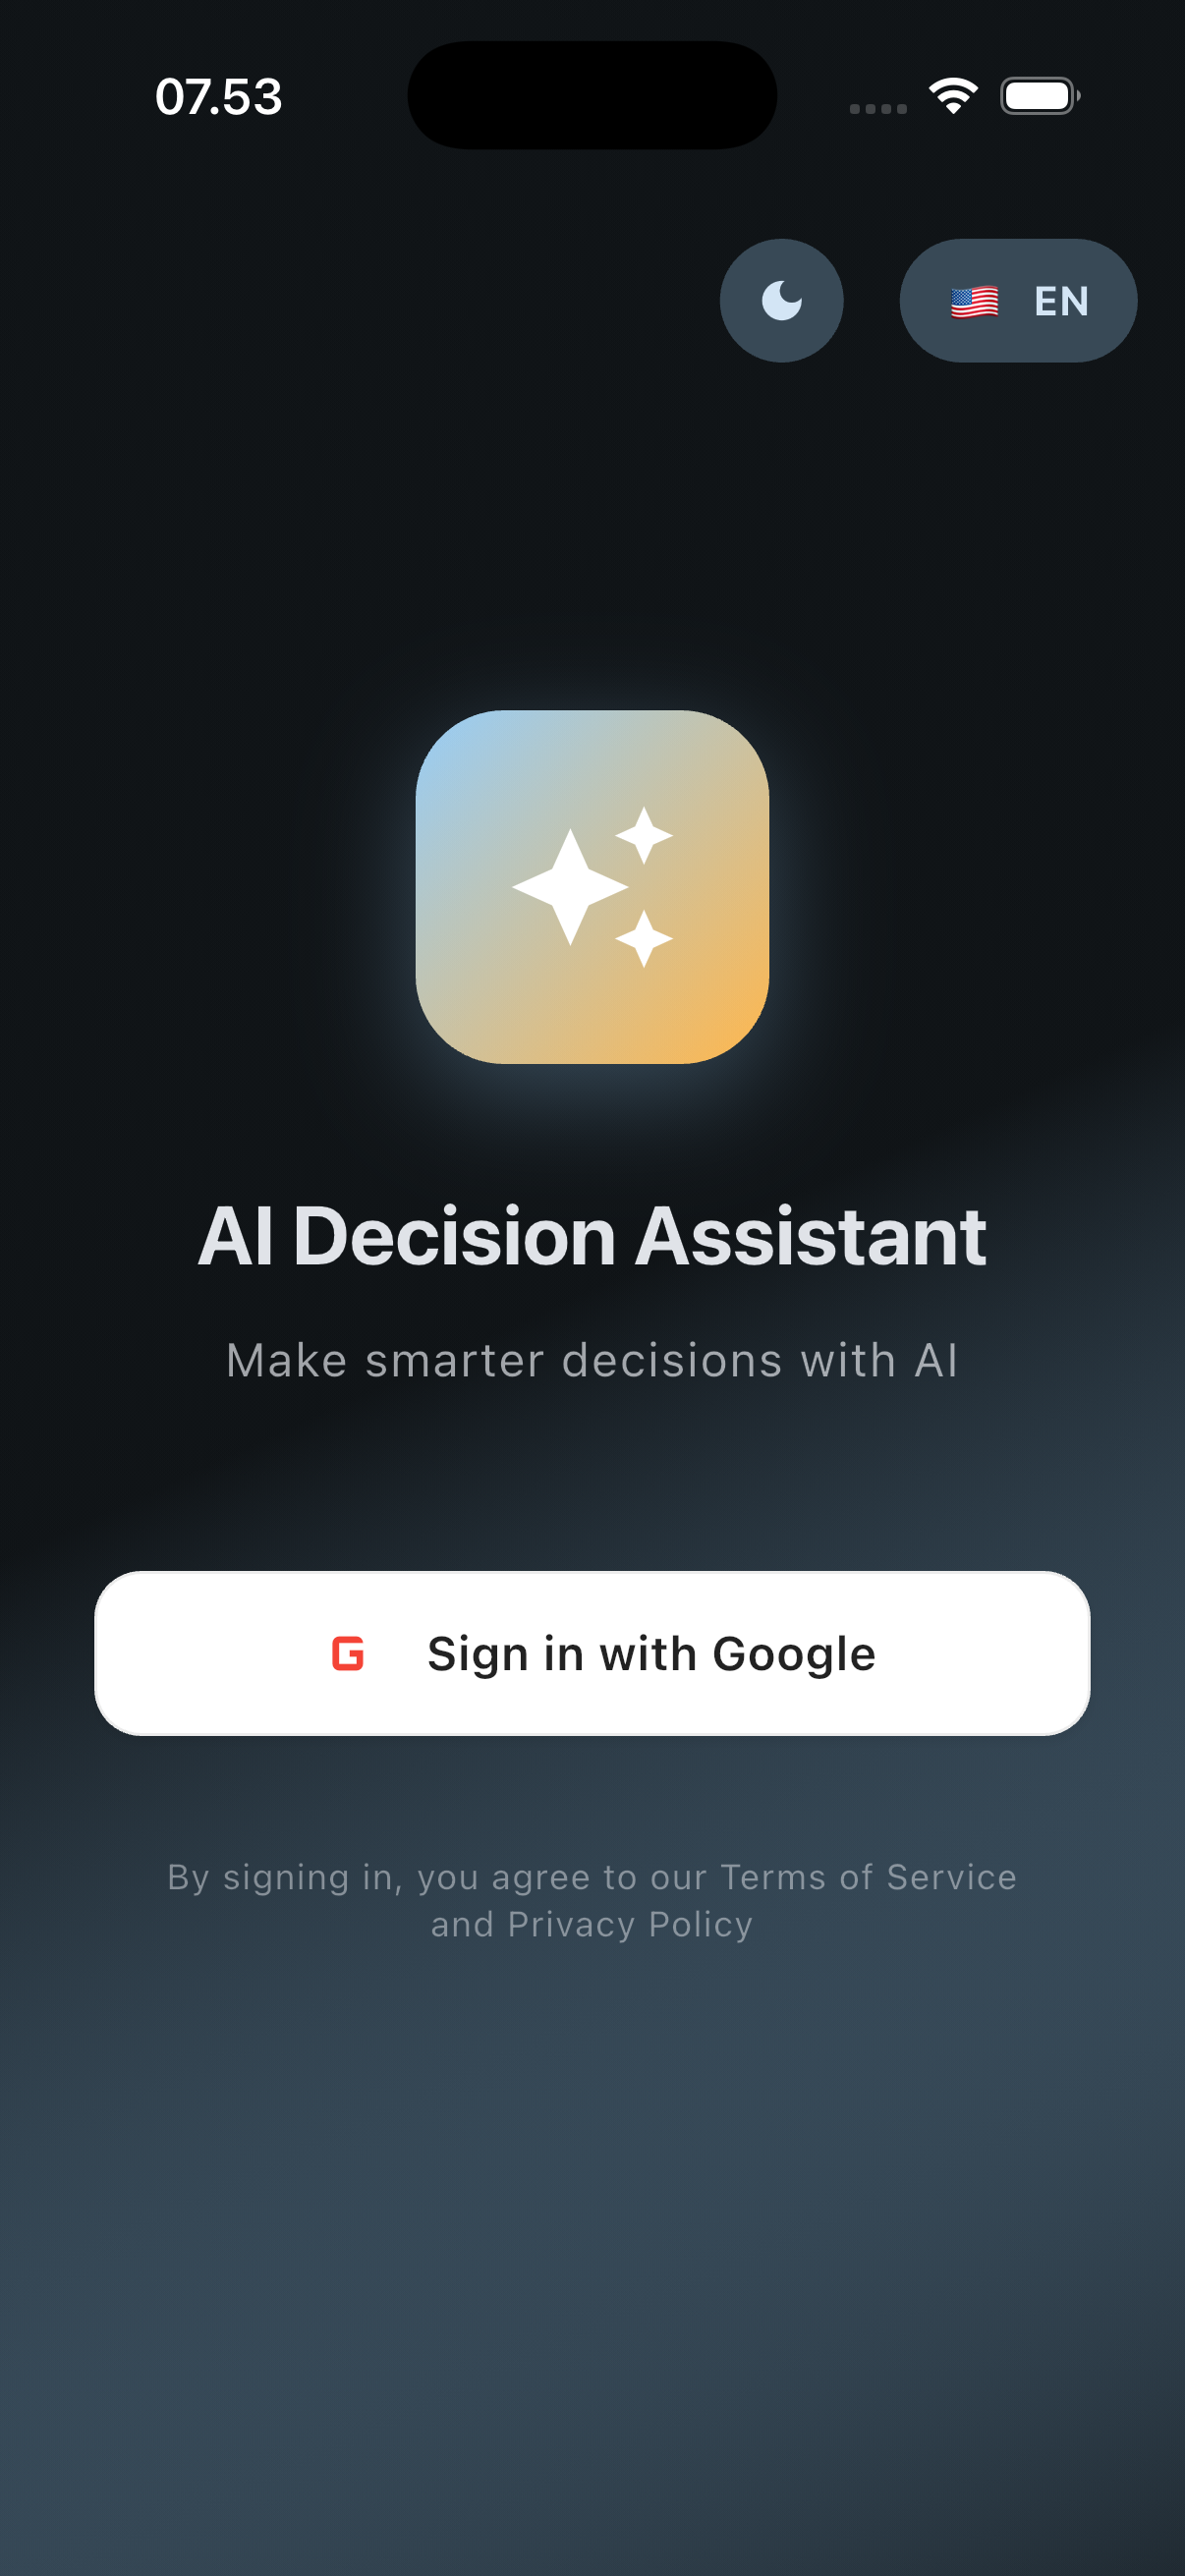
\includegraphics[width=\linewidth]{ss01_login.png}
    \caption*{(a) Halaman login aplikasi}
  \end{minipage}\hfill
  \begin{minipage}{0.47\textwidth}
    \centering
    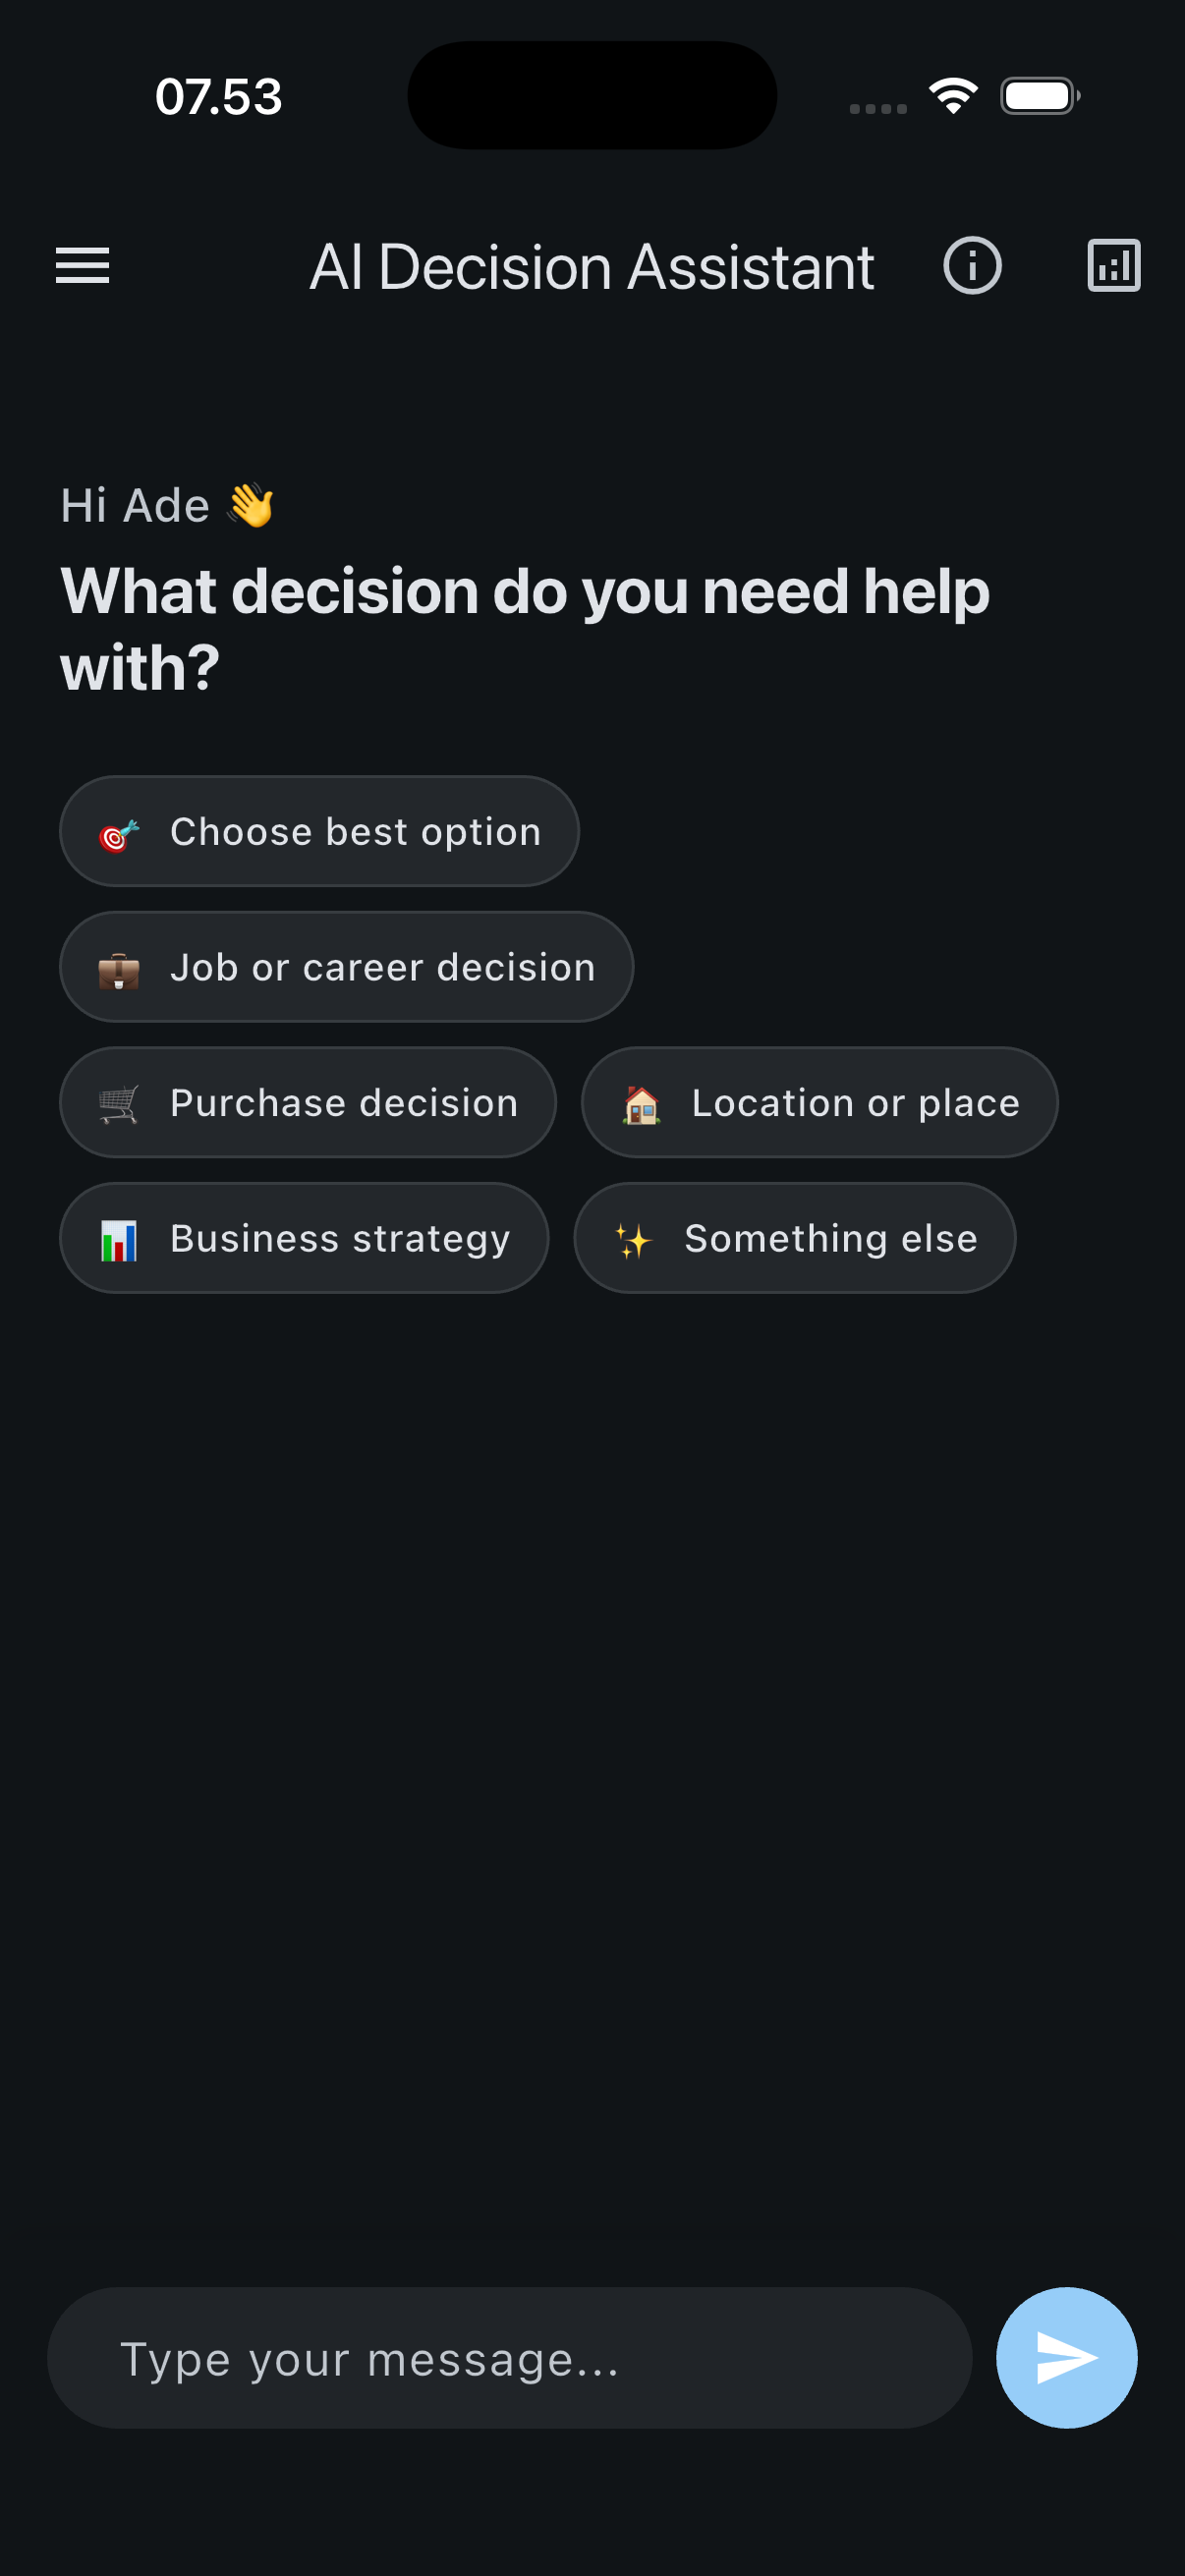
\includegraphics[width=\linewidth]{ss02_chat_awal.png}
    \caption*{(b) Halaman chat awal}
  \end{minipage}
  \caption{Tampilan awal sistem AI Assisted DSS}
\end{figure}

\begin{figure}[H]
  \centering
  \begin{minipage}{0.47\textwidth}
    \centering
    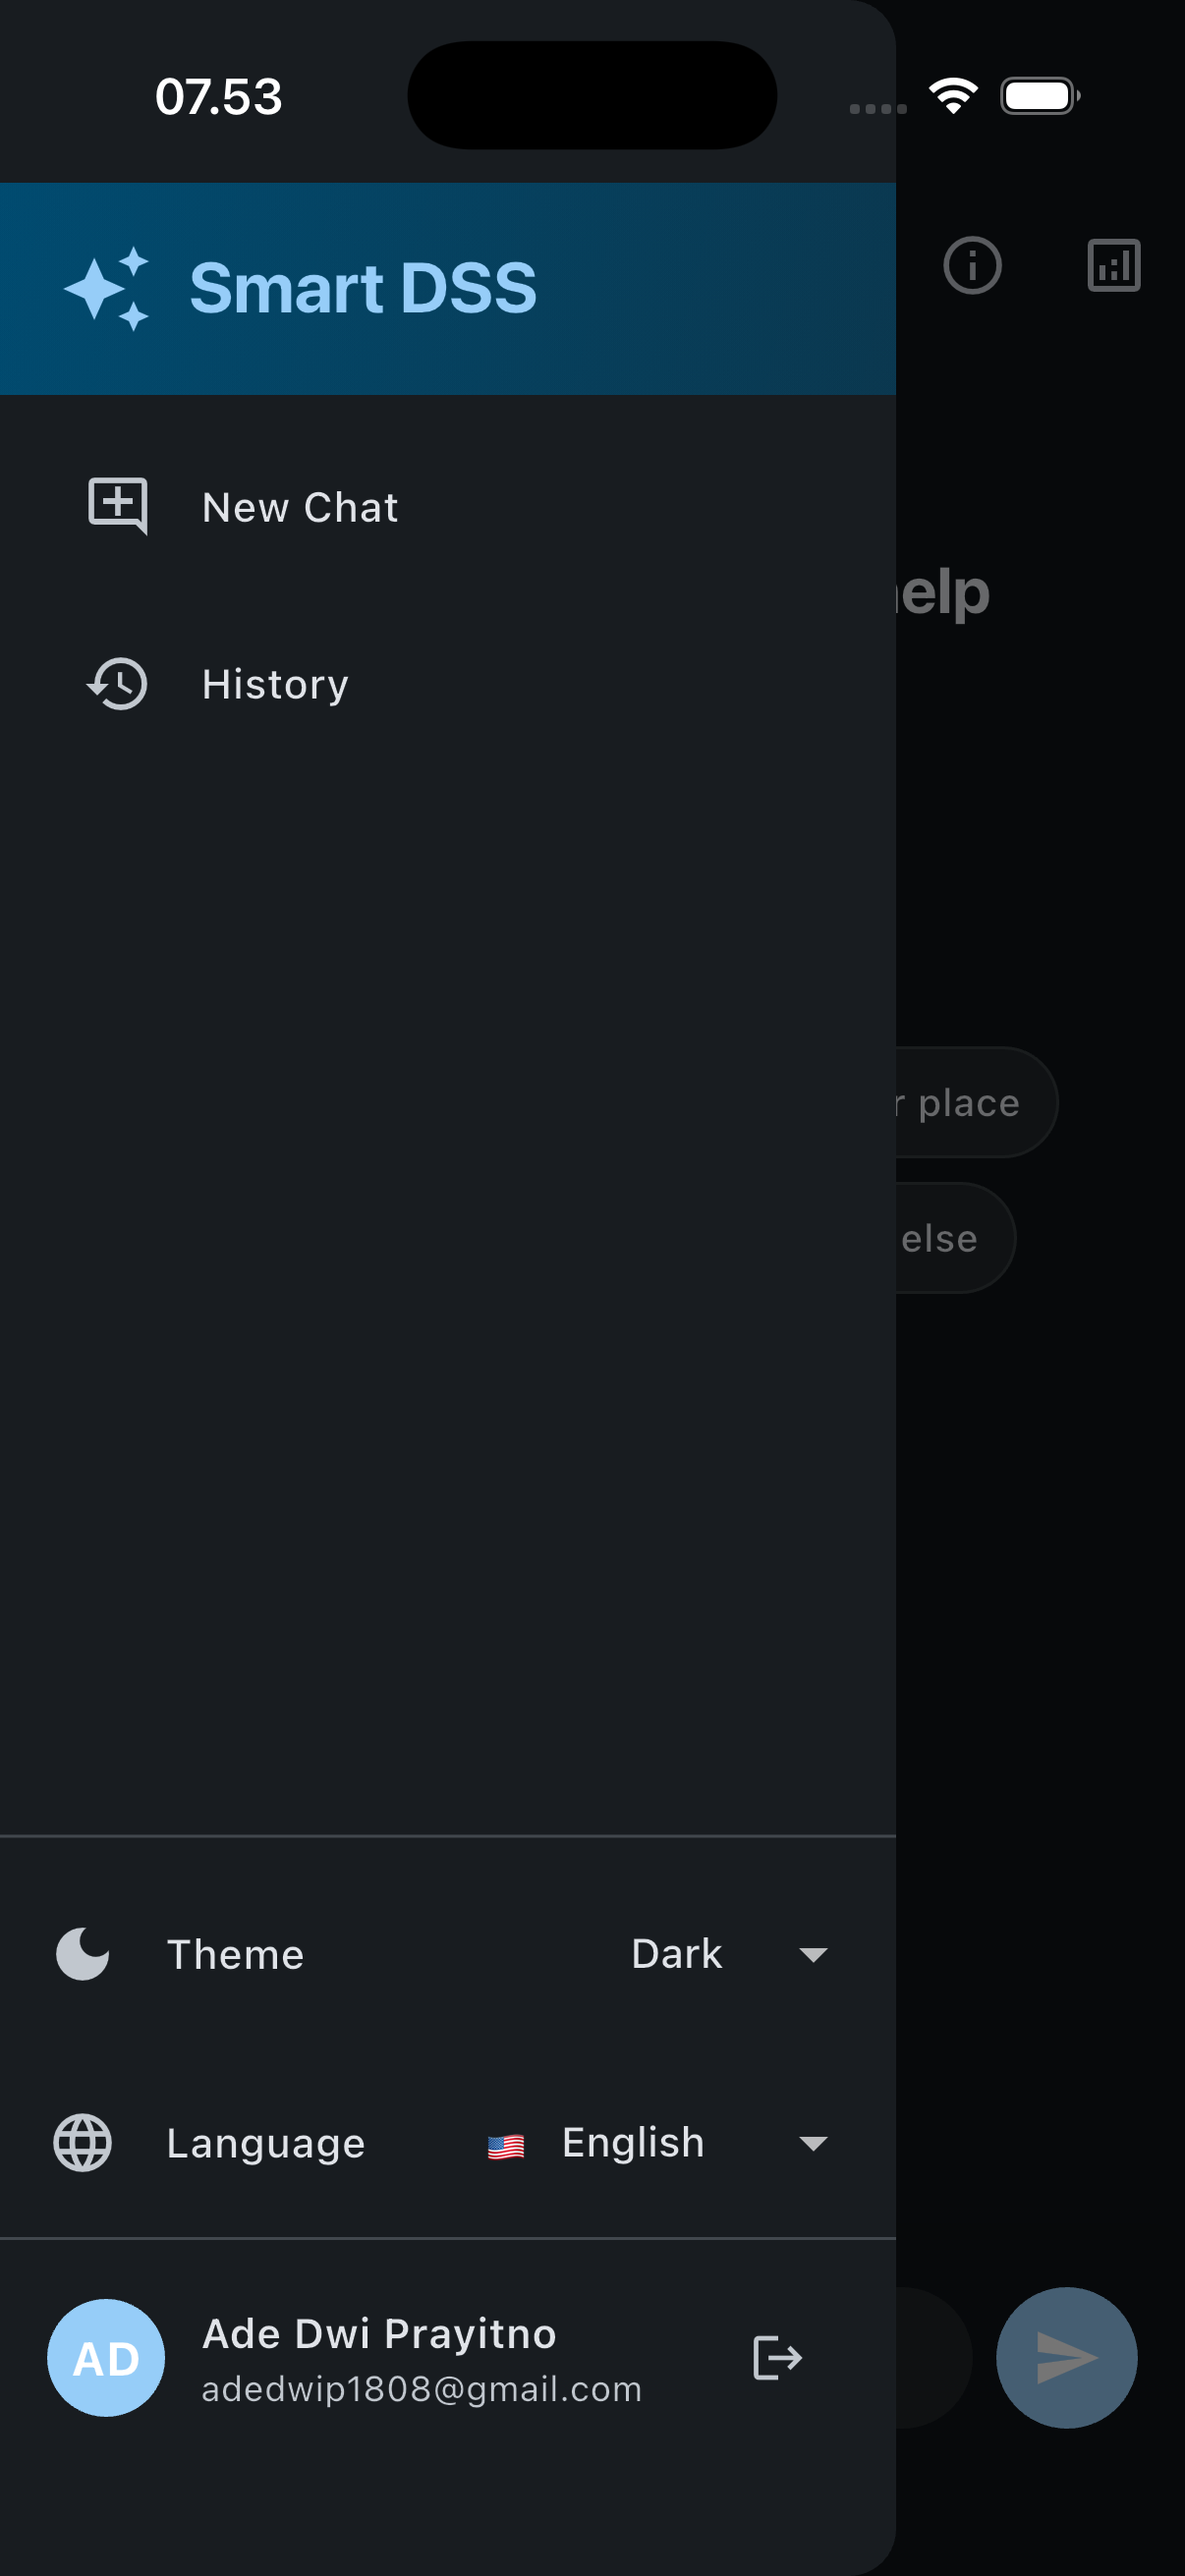
\includegraphics[width=\linewidth]{ss03_menu_samping.png}
    \caption*{(a) Menu samping aplikasi}
  \end{minipage}\hfill
  \begin{minipage}{0.47\textwidth}
    \centering
    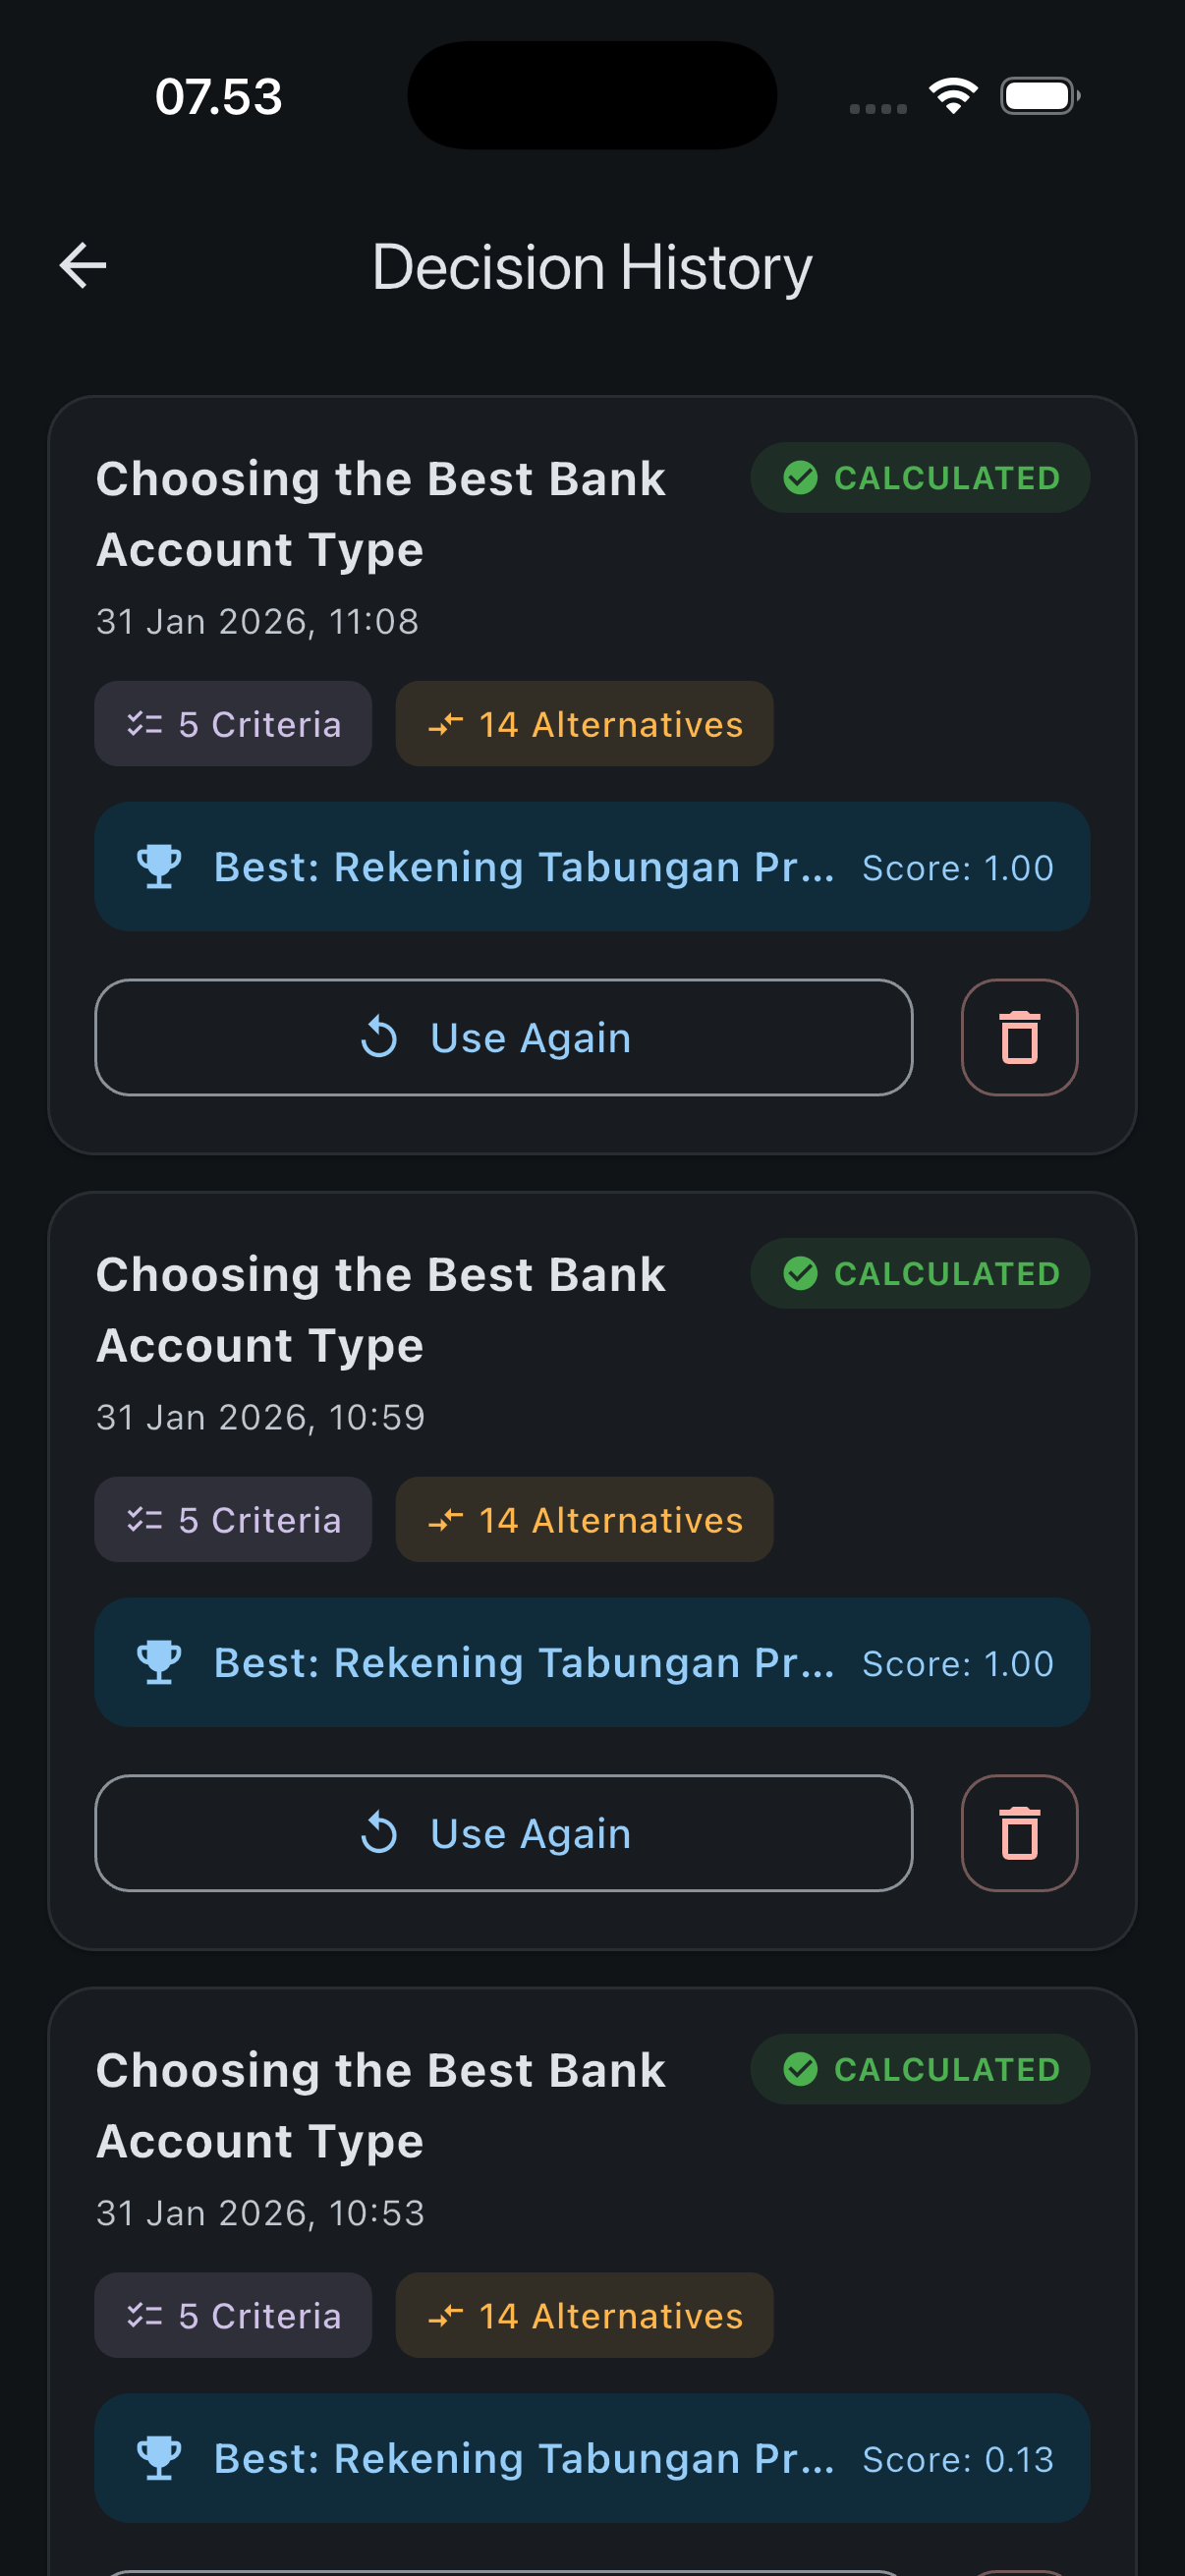
\includegraphics[width=\linewidth]{ss04_riwayat.png}
    \caption*{(b) Halaman riwayat keputusan}
  \end{minipage}
  \caption{Navigasi utama dan manajemen riwayat keputusan}
\end{figure}

Antarmuka awal menunjukkan bahwa aplikasi mendukung autentikasi pengguna, percakapan terarah, serta navigasi menuju fitur riwayat. Fitur ini penting untuk menjaga kontinuitas proses pengambilan keputusan yang biasanya bersifat iteratif.

\subsection{Hasil Perhitungan dan Analisis}
\begin{figure}[H]
  \centering
  \begin{minipage}{0.47\textwidth}
    \centering
    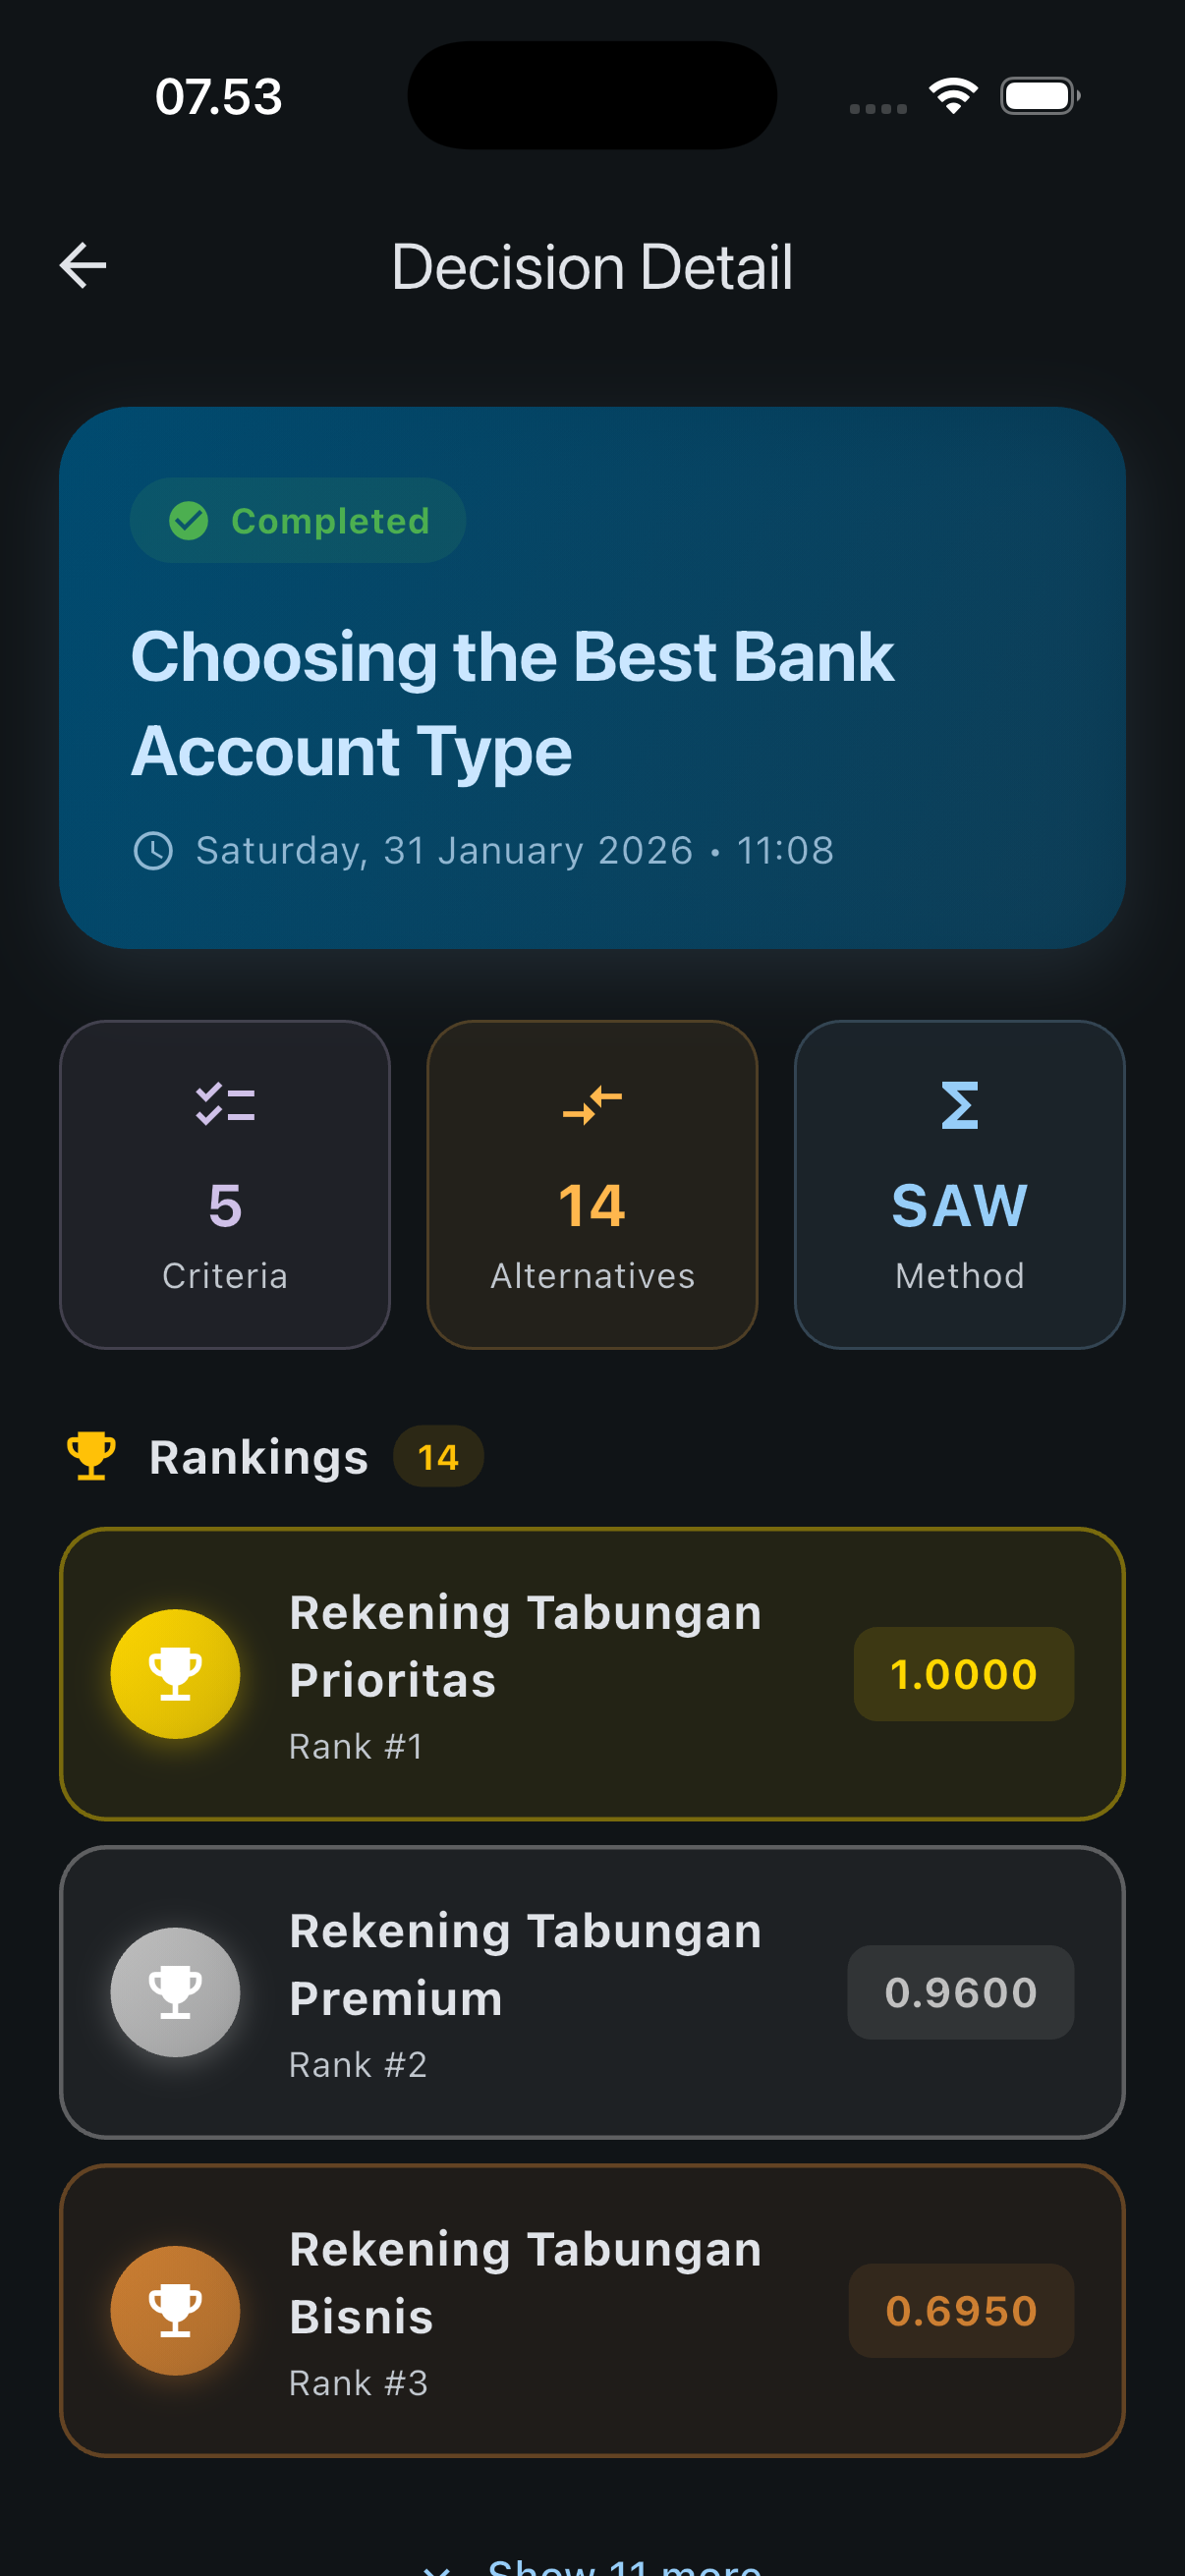
\includegraphics[width=\linewidth]{ss05_detail_hasil_saw.png}
    \caption*{(a) Detail hasil peringkat (SAW)}
  \end{minipage}\hfill
  \begin{minipage}{0.47\textwidth}
    \centering
    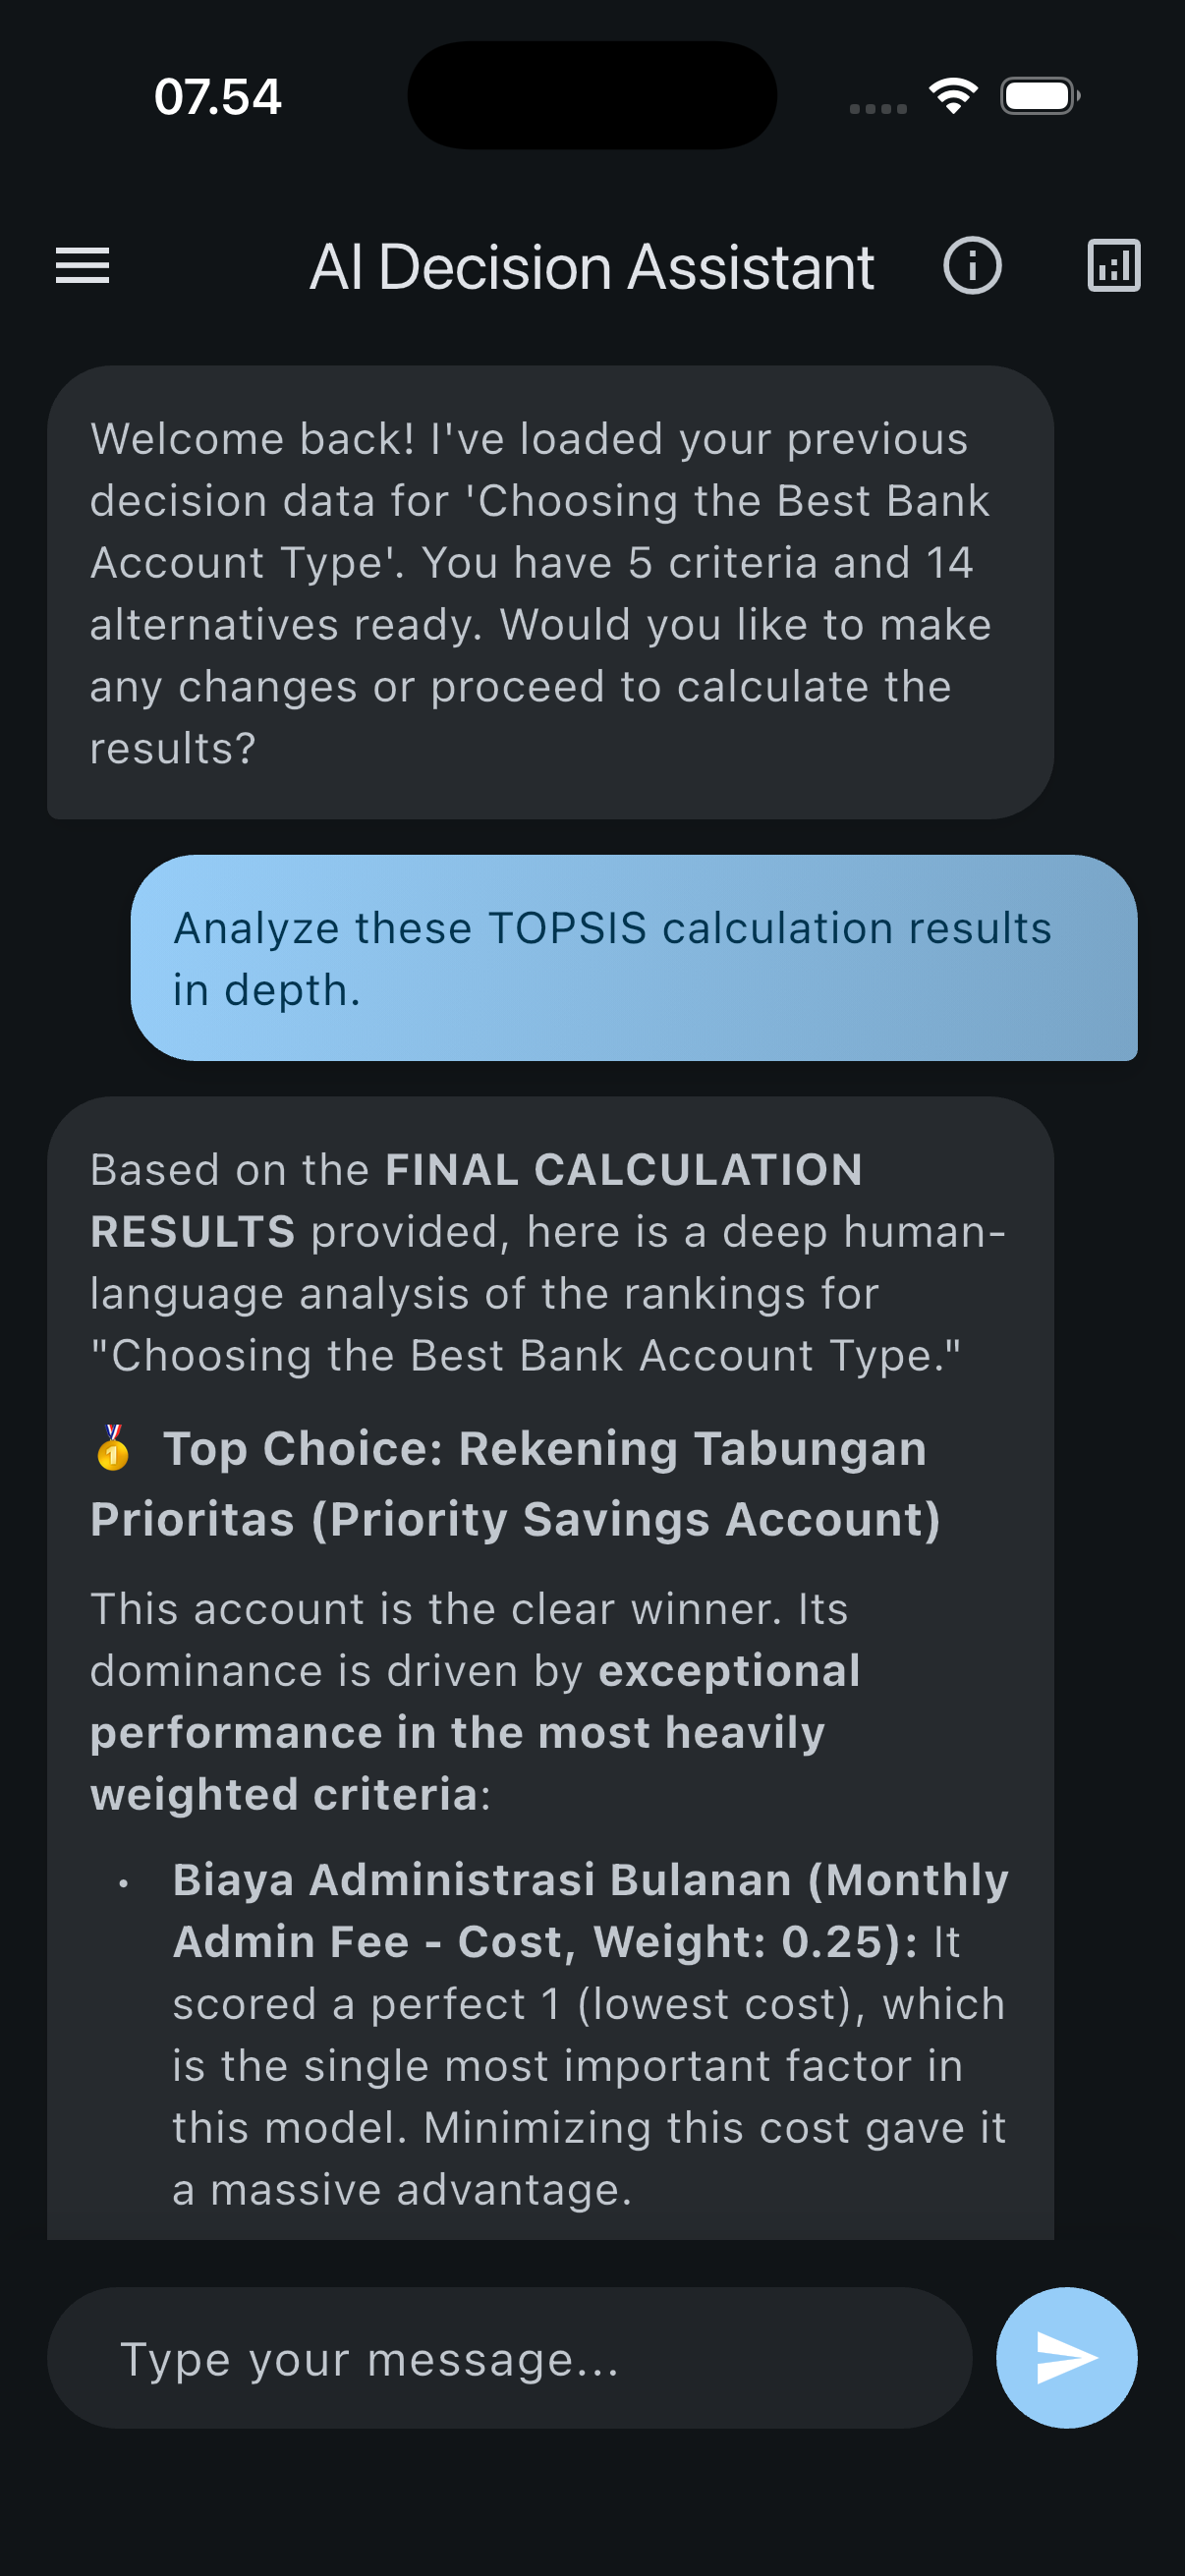
\includegraphics[width=\linewidth]{ss06_analisis_ai_topsis.png}
    \caption*{(b) Analisis naratif AI atas hasil}
  \end{minipage}
  \caption{Output ranking dan interpretasi hasil}
\end{figure}

\begin{figure}[H]
  \centering
  \begin{minipage}{0.47\textwidth}
    \centering
    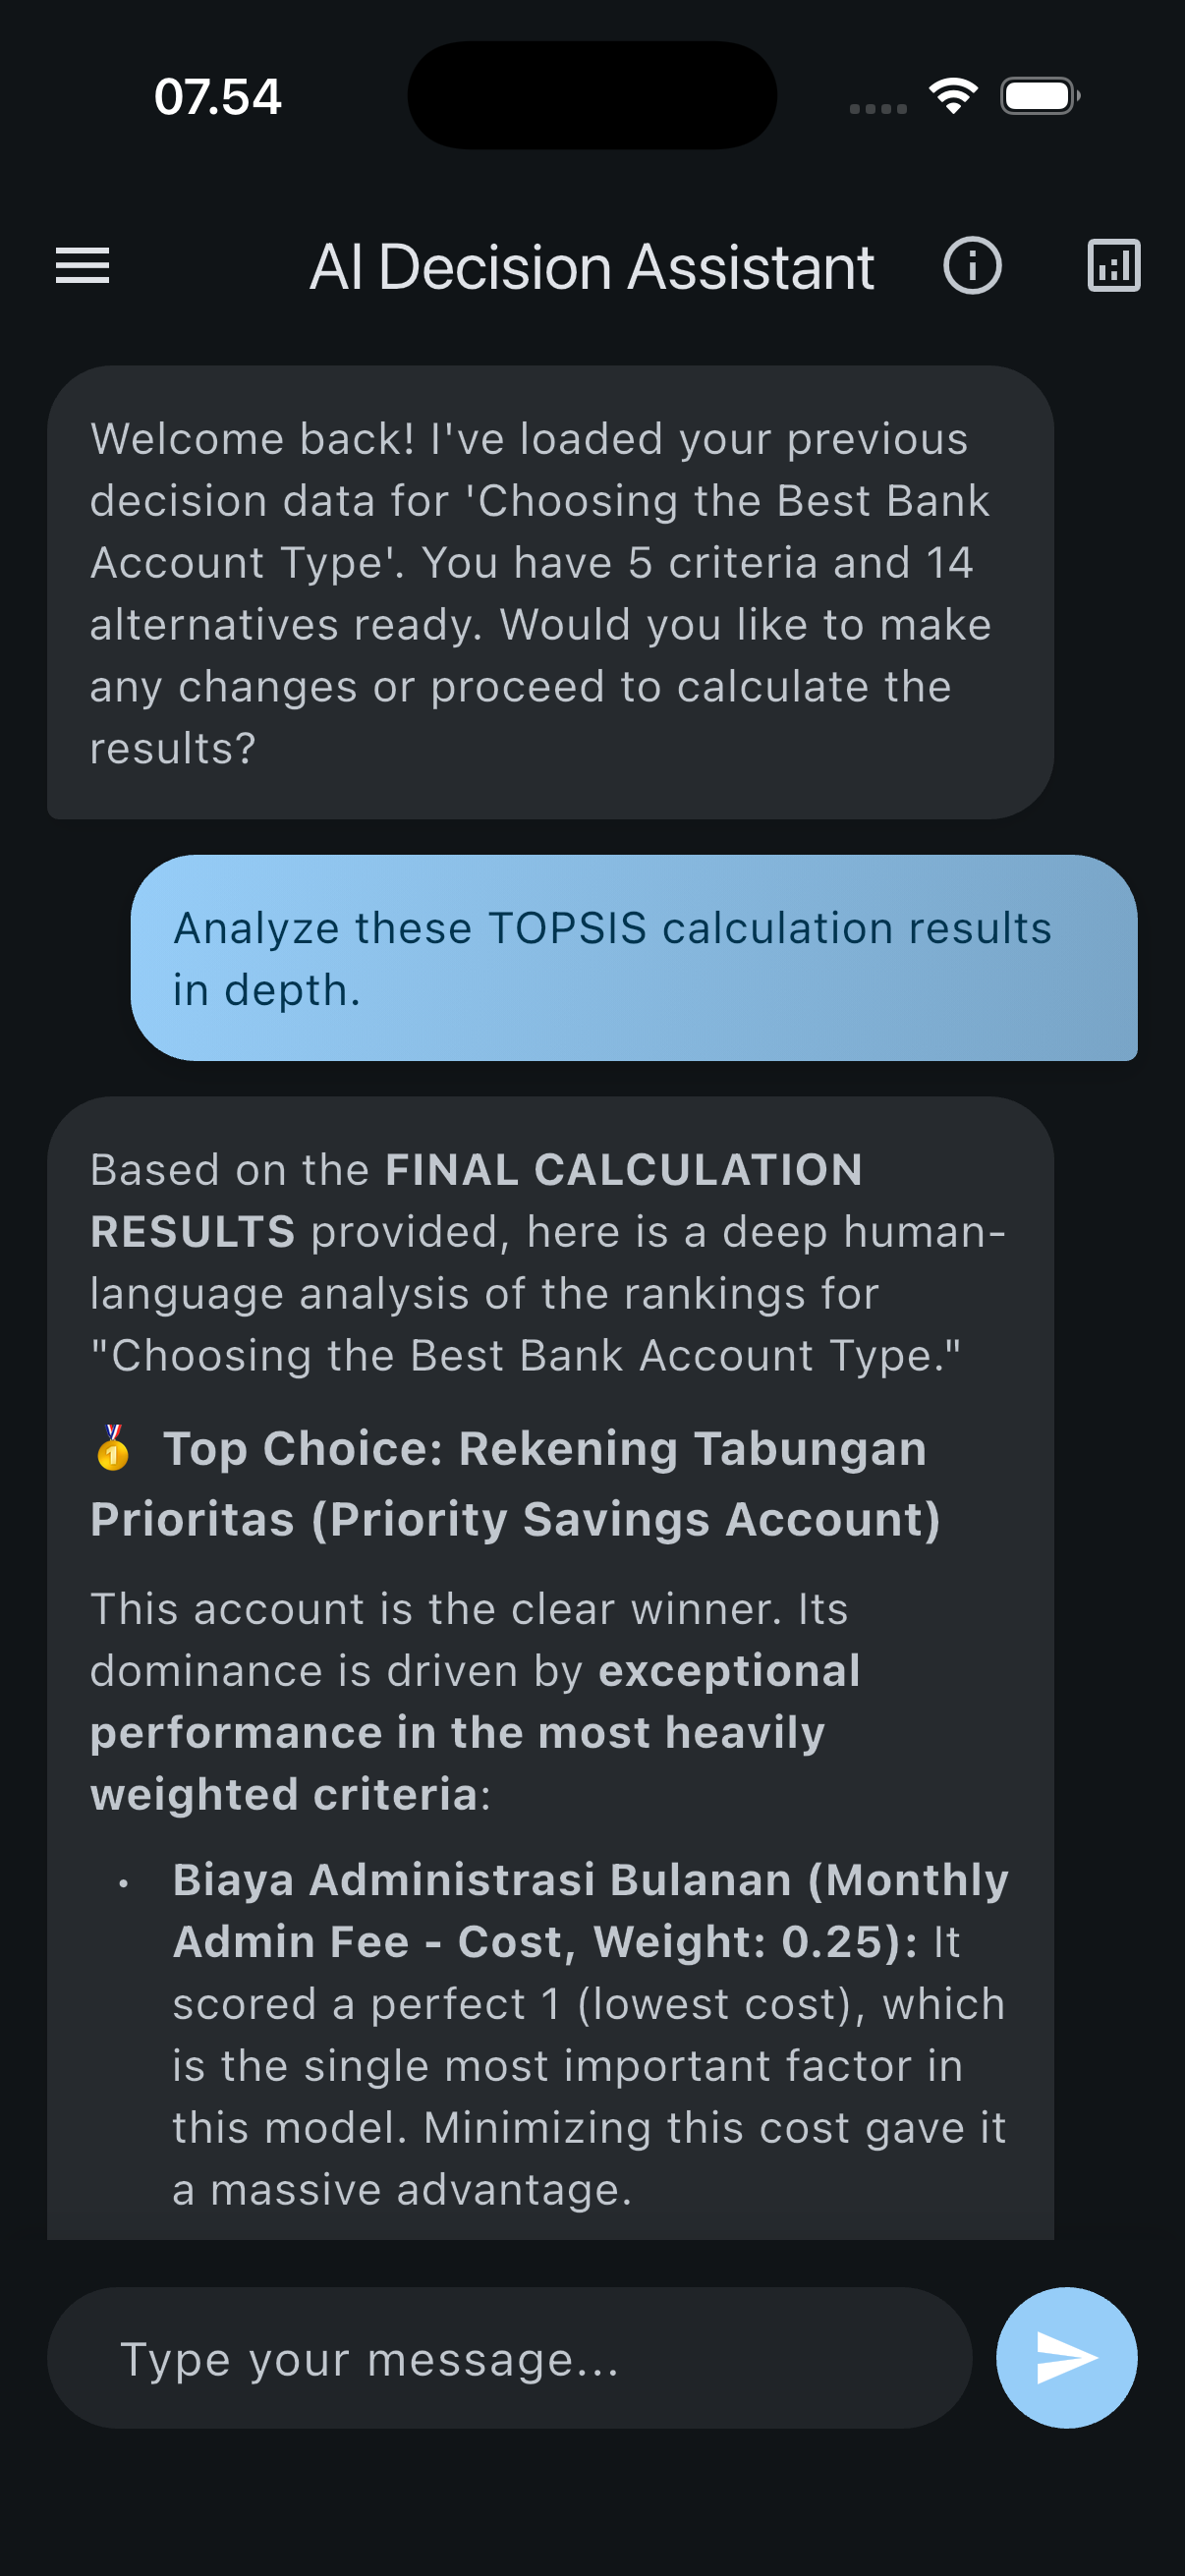
\includegraphics[width=\linewidth]{ss07_analisis_ai_topsis_alt.png}
    \caption*{(a) Variasi tampilan analisis chat}
  \end{minipage}\hfill
  \begin{minipage}{0.47\textwidth}
    \centering
    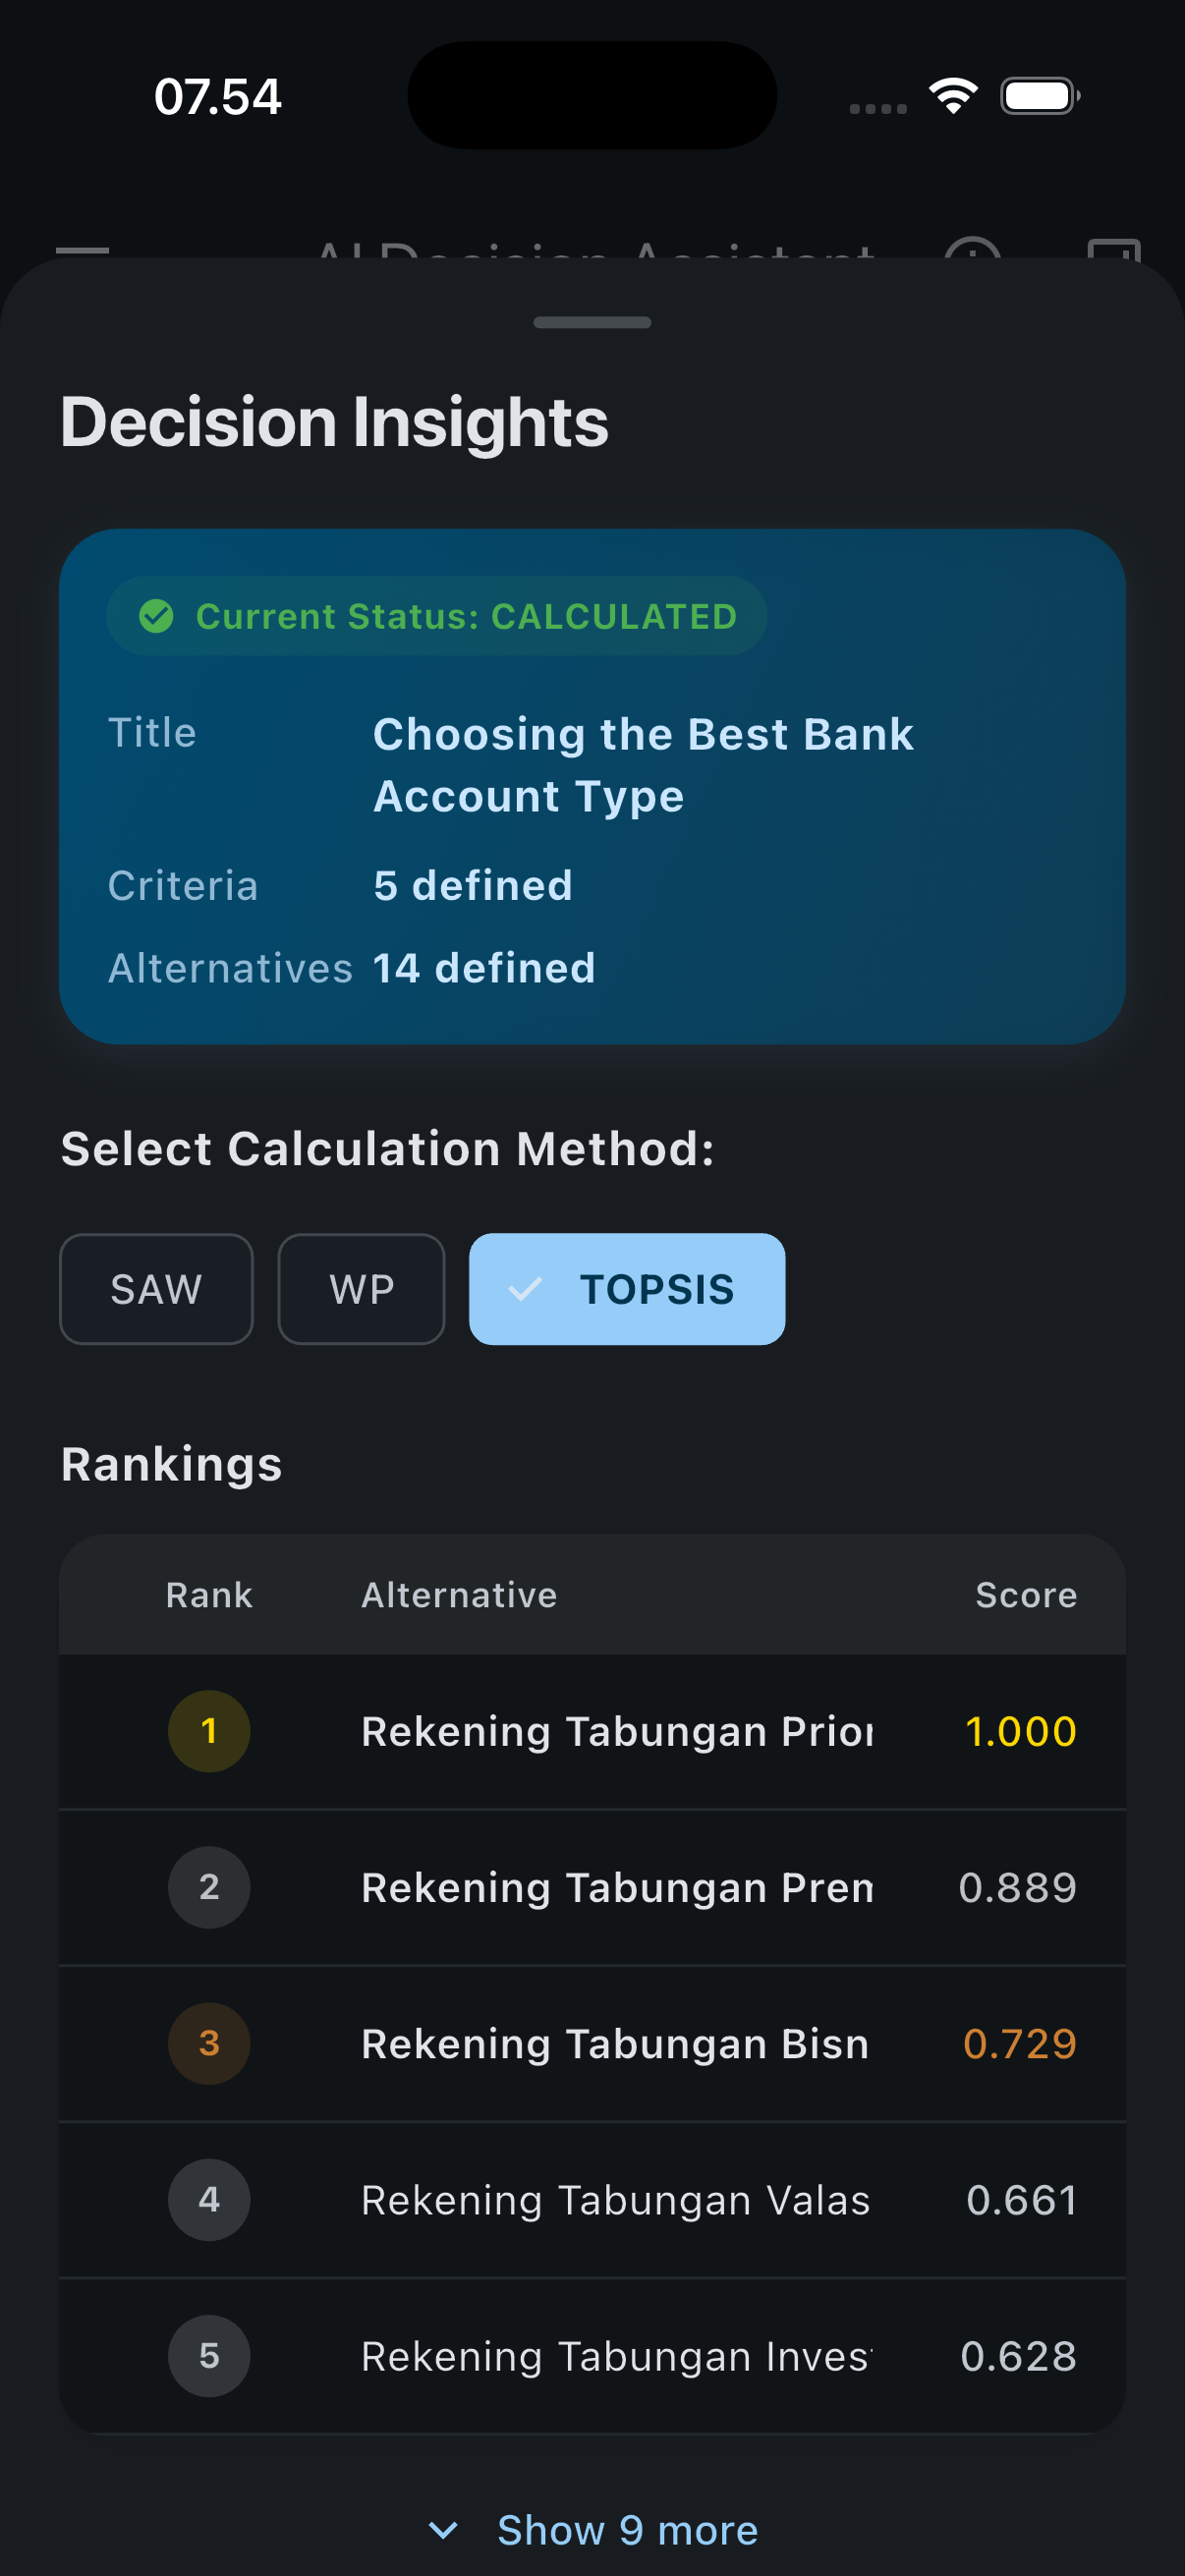
\includegraphics[width=\linewidth]{ss08_insight_topsis.png}
    \caption*{(b) Insight perhitungan metode TOPSIS}
  \end{minipage}
  \caption{Analisis AI dan pemilihan metode perhitungan}
\end{figure}

\begin{figure}[H]
  \centering
  \begin{minipage}{0.47\textwidth}
    \centering
    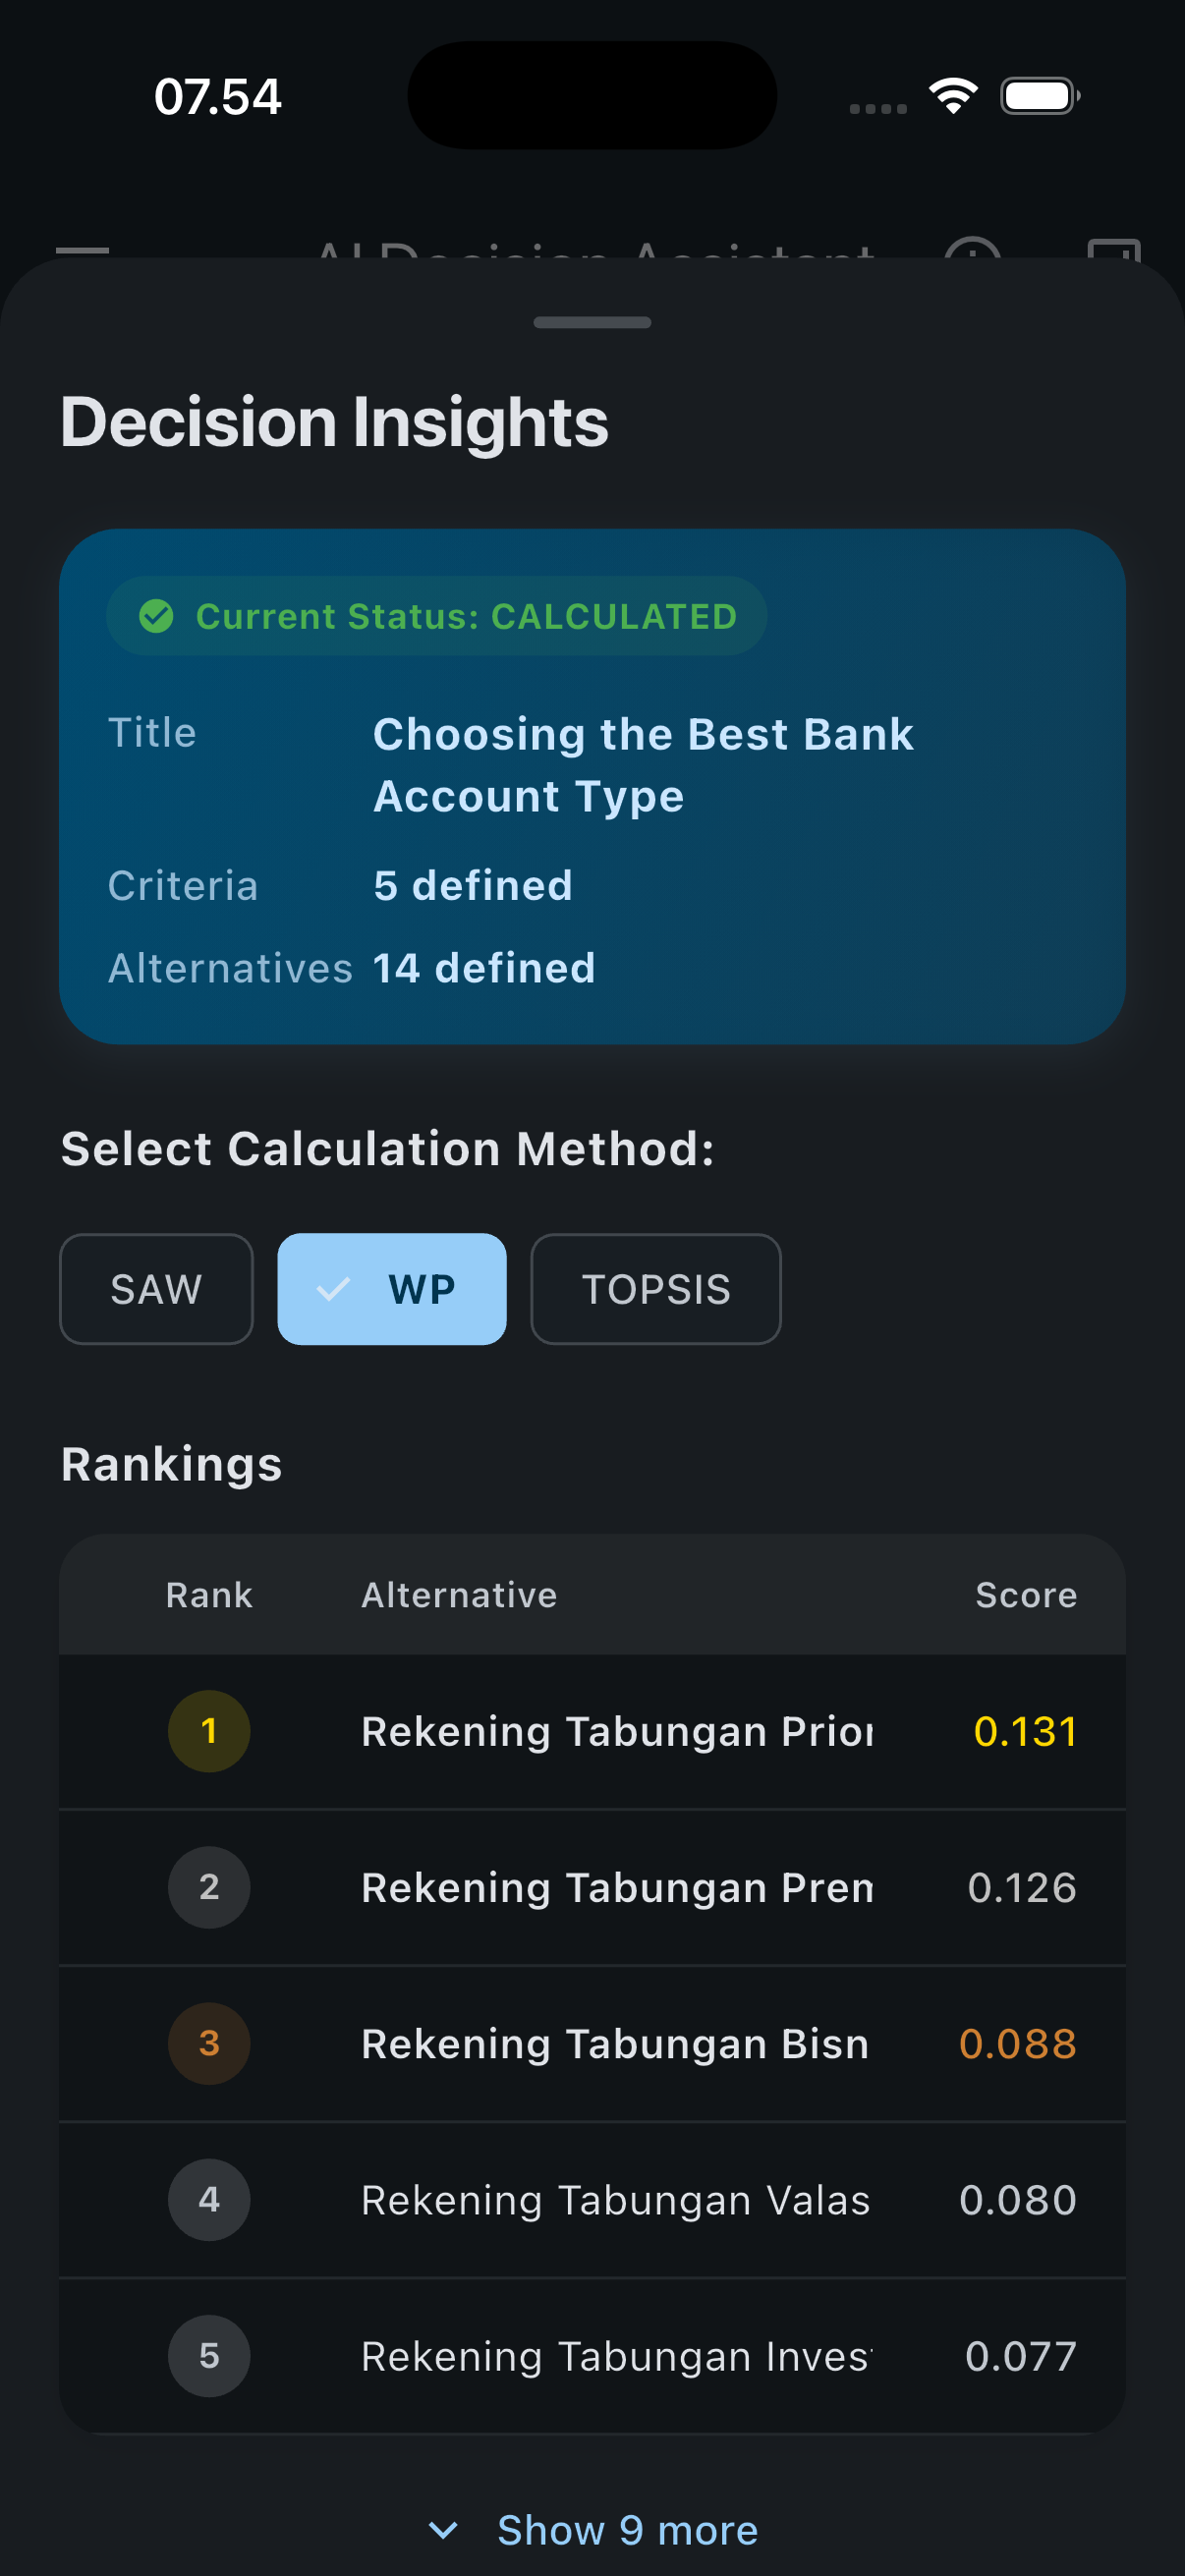
\includegraphics[width=\linewidth]{ss09_insight_wp.png}
    \caption*{(a) Insight perhitungan metode WP}
  \end{minipage}\hfill
  \begin{minipage}{0.47\textwidth}
    \centering
    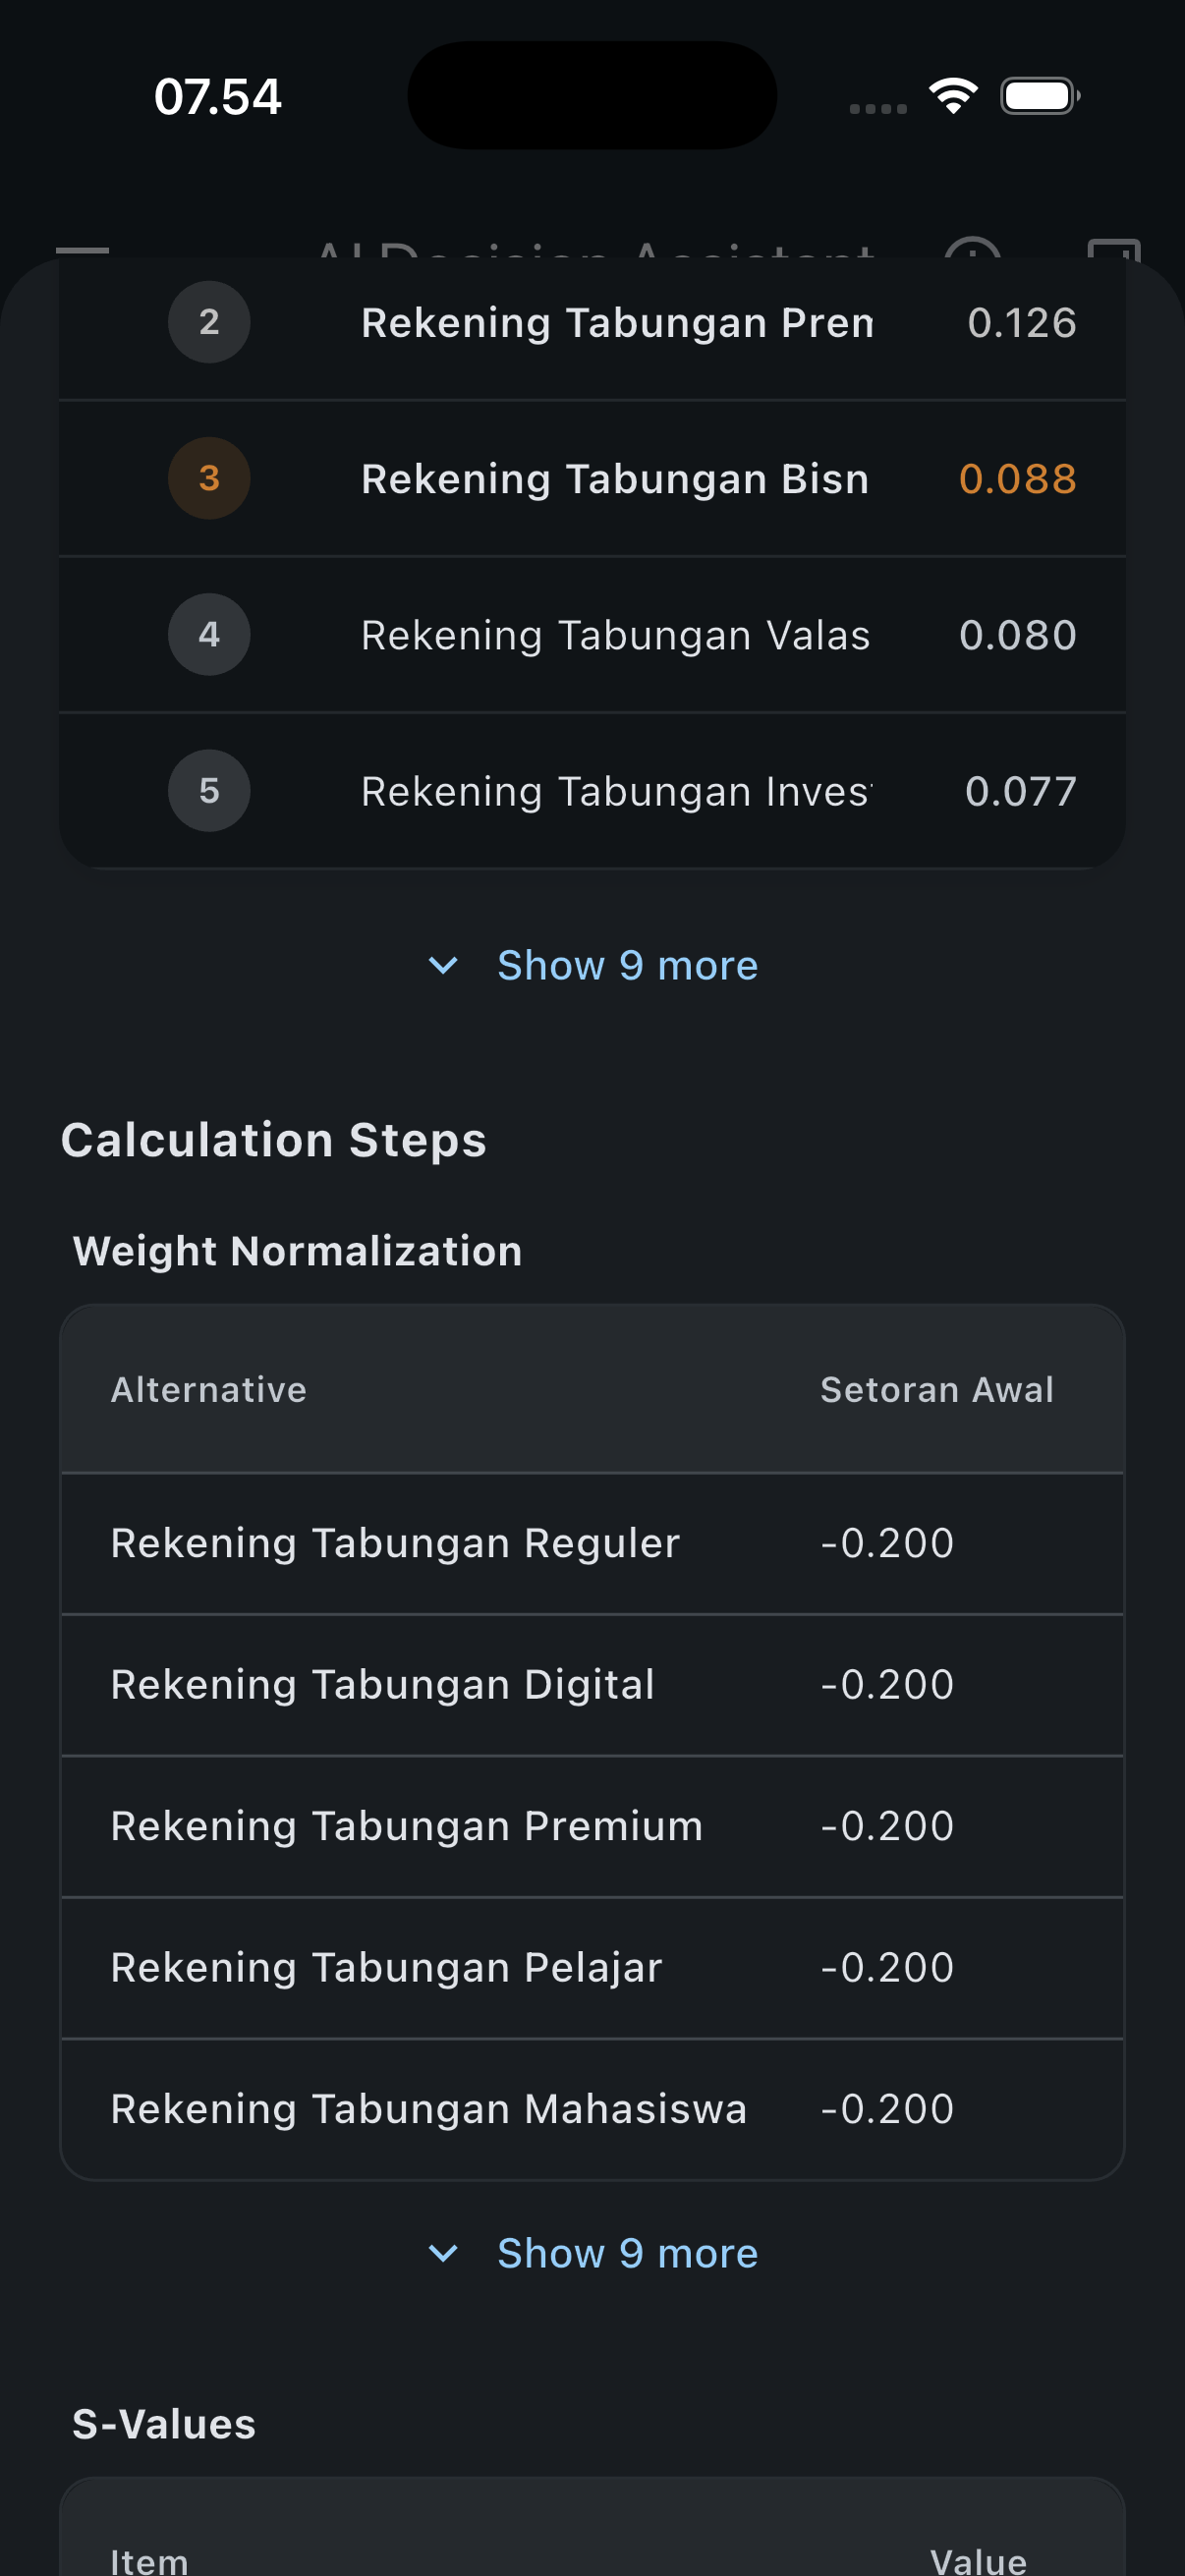
\includegraphics[width=\linewidth]{ss10_langkah_wp.png}
    \caption*{(b) Langkah/matriks perhitungan WP}
  \end{minipage}
  \caption{Perbandingan hasil dan detail analitik antar metode}
\end{figure}

Hasil implementasi menunjukkan:
\begin{enumerate}
  \item Sistem mampu menyimpan data keputusan dan memanggil ulang untuk analisis lanjutan.
  \item Ranking alternatif ditampilkan konsisten pada berbagai metode.
  \item Pengguna dapat melihat matriks perhitungan untuk verifikasi teknis.
  \item AI memberi penjelasan bahasa natural yang membantu interpretasi hasil akhir.
\end{enumerate}

\section{Diskusi Bug dan Perbaikan Implementasi}
\subsection{Deskripsi Bug yang Ditemukan}
Setelah sesi diskusi dan pengujian lanjutan, ditemukan bug pada konsistensi hasil: nilai atau narasi peringkat yang disampaikan AI di area chat kadang tidak sama dengan nilai yang tampil pada panel sidebar \textit{Decision Insights}. Gejala ini muncul terutama saat pengguna meminta analisis mendalam setelah hasil kalkulasi sudah tersedia. Dalam beberapa kasus, AI membentuk narasi seolah-olah melakukan perhitungan baru secara mandiri, padahal sumber nilai resmi seharusnya berasal dari mesin DSS internal aplikasi.

Kondisi ini penting karena aplikasi SPK menuntut konsistensi dan keterlacakan keputusan. Ketika pengguna melihat dua representasi nilai yang berbeda pada satu sesi yang sama, kepercayaan terhadap sistem dapat menurun walaupun perhitungan inti sebenarnya sudah benar.

\subsection{Analisis Akar Masalah}
Analisis menunjukkan bahwa akar masalah bukan pada algoritma SAW/WP/TOPSIS, melainkan pada lapisan generatif AI saat menyusun penjelasan. Tanpa arahan yang cukup ketat, model bahasa dapat mencoba melakukan estimasi sendiri berdasarkan konteks teks, bukan murni menyalin hasil final dari mesin perhitungan.

Secara fungsional, sistem memiliki dua komponen yang berbeda:
\begin{enumerate}
  \item Mesin DSS deterministik yang menghasilkan ranking dan skor final.
  \item AI asisten percakapan yang bertugas menjelaskan hasil kepada pengguna.
\end{enumerate}
Pada kondisi tertentu, komponen kedua dapat melampaui perannya jika tidak dibatasi dengan aturan prompt dan konteks data yang tegas.

\subsection{Perbaikan yang Sudah Diimplementasikan}
Perbaikan pasca-diskusi telah diimplementasikan dengan prinsip \textit{single source of truth}, yaitu semua narasi hasil harus merujuk ke keluaran final mesin DSS. Perbaikan ini meliputi:
\begin{enumerate}
  \item Instruksi sistem AI dipertegas agar AI tidak melakukan kalkulasi mandiri.
  \item Hasil akhir peringkat (\textit{final calculation results}) selalu disuntikkan ke konteks percakapan sebelum AI menyusun respons.
  \item AI diarahkan untuk berfokus pada penjelasan alasan ranking (interpretasi), bukan menghasilkan angka baru.
  \item Aplikasi tetap menyediakan panel analitik sebagai titik verifikasi teknis ketika pengguna ingin memeriksa detail matriks.
\end{enumerate}

Dengan pendekatan ini, chat berfungsi sebagai lapisan interpretatif, sedangkan sidebar tetap menjadi representasi numerik resmi. Pemisahan peran ini menjaga akurasi, transparansi, dan pengalaman pengguna secara bersamaan.

\subsection{Validasi Pasca-Perbaikan}
Untuk memastikan bug telah tertangani, dilakukan validasi dengan beberapa skenario penggunaan normal. Tolok ukur utama adalah kesesuaian antara narasi chat dan nilai ranking di panel \textit{Decision Insights}.

\begin{table}[H]
  \centering
  \caption{Ringkasan validasi konsistensi nilai setelah perbaikan}
  \small
  \begin{tabular}{p{0.08\textwidth} p{0.28\textwidth} p{0.30\textwidth} p{0.20\textwidth}}
    \toprule
    No & Skenario Uji & Indikator Keberhasilan & Hasil \\
    \midrule
    1 & Hitung awal metode SAW pada data lengkap & Narasi chat menyebut pemenang yang sama dengan panel ranking SAW & Sesuai \\
    2 & Ganti metode ke WP pada sesi yang sama & Urutan alternatif top-3 di chat sama dengan sidebar WP & Sesuai \\
    3 & Ganti metode ke TOPSIS lalu minta analisis mendalam & Skor referensi di chat tidak bertentangan dengan panel TOPSIS & Sesuai \\
    4 & Muat ulang sesi dari riwayat lalu minta penjelasan ulang & AI tetap merujuk hasil kalkulasi tersimpan, bukan menghitung ulang & Sesuai \\
    \bottomrule
  \end{tabular}
\end{table}

Perbaikan ini meningkatkan reliabilitas aplikasi karena semua angka keputusan kembali dikunci pada hasil mesin DSS sebagai sumber otoritatif. Chat difungsikan sebagai lapisan interpretasi, bukan kalkulasi, sehingga konsistensi output antar tampilan lebih terjaga.

\section{Kesimpulan dan Saran}
\subsection{Kesimpulan}
Berdasarkan implementasi yang telah dilakukan, aplikasi \textit{AI Assisted DSS} berhasil memenuhi tujuan tugas, yaitu menyediakan dukungan pengambilan keputusan berbasis metode SAW, WP, dan TOPSIS dengan antarmuka percakapan AI yang terstruktur. Integrasi ini membuat proses input data keputusan lebih mudah, sementara hasil perhitungan tetap transparan karena dikerjakan oleh modul DSS lokal.

\subsection{Saran Pengembangan}
\begin{enumerate}
  \item Menambahkan evaluasi kuantitatif akurasi rekomendasi berbasis studi kasus nyata.
  \item Menambahkan ekspor laporan keputusan ke format PDF secara otomatis dari aplikasi.
  \item Menyediakan dashboard visual perbandingan sensitivitas bobot tiap kriteria.
\end{enumerate}

\section{Tech Stack dan Link Repository}
\subsection{Tech Stack}
\begin{enumerate}
  \item Flutter (framework pengembangan aplikasi lintas platform).
  \item Firebase Firestore (penyimpanan data sesi keputusan dan riwayat).
  \item DeepSeek API (asisten AI untuk alur percakapan pengumpulan data keputusan).
  \item Riverpod (manajemen state aplikasi).
  \item Metode DSS: SAW, WP, dan TOPSIS (mesin perhitungan keputusan).
\end{enumerate}

\subsection{Link Repository}
Repositori proyek dapat diakses melalui tautan berikut:
\begin{center}
  \url{https://github.com/prima101112/ai-asisted-dss}
\end{center}

\end{document}
